% Options for packages loaded elsewhere
% Options for packages loaded elsewhere
\PassOptionsToPackage{unicode}{hyperref}
\PassOptionsToPackage{hyphens}{url}
\PassOptionsToPackage{dvipsnames,svgnames,x11names}{xcolor}
%
\documentclass[
  letterpaper,
  DIV=11,
  numbers=noendperiod]{scrartcl}
\usepackage{xcolor}
\usepackage{amsmath,amssymb}
\setcounter{secnumdepth}{-\maxdimen} % remove section numbering
\usepackage{iftex}
\ifPDFTeX
  \usepackage[T1]{fontenc}
  \usepackage[utf8]{inputenc}
  \usepackage{textcomp} % provide euro and other symbols
\else % if luatex or xetex
  \usepackage{unicode-math} % this also loads fontspec
  \defaultfontfeatures{Scale=MatchLowercase}
  \defaultfontfeatures[\rmfamily]{Ligatures=TeX,Scale=1}
\fi
\usepackage{lmodern}
\ifPDFTeX\else
  % xetex/luatex font selection
\fi
% Use upquote if available, for straight quotes in verbatim environments
\IfFileExists{upquote.sty}{\usepackage{upquote}}{}
\IfFileExists{microtype.sty}{% use microtype if available
  \usepackage[]{microtype}
  \UseMicrotypeSet[protrusion]{basicmath} % disable protrusion for tt fonts
}{}
\makeatletter
\@ifundefined{KOMAClassName}{% if non-KOMA class
  \IfFileExists{parskip.sty}{%
    \usepackage{parskip}
  }{% else
    \setlength{\parindent}{0pt}
    \setlength{\parskip}{6pt plus 2pt minus 1pt}}
}{% if KOMA class
  \KOMAoptions{parskip=half}}
\makeatother
% Make \paragraph and \subparagraph free-standing
\makeatletter
\ifx\paragraph\undefined\else
  \let\oldparagraph\paragraph
  \renewcommand{\paragraph}{
    \@ifstar
      \xxxParagraphStar
      \xxxParagraphNoStar
  }
  \newcommand{\xxxParagraphStar}[1]{\oldparagraph*{#1}\mbox{}}
  \newcommand{\xxxParagraphNoStar}[1]{\oldparagraph{#1}\mbox{}}
\fi
\ifx\subparagraph\undefined\else
  \let\oldsubparagraph\subparagraph
  \renewcommand{\subparagraph}{
    \@ifstar
      \xxxSubParagraphStar
      \xxxSubParagraphNoStar
  }
  \newcommand{\xxxSubParagraphStar}[1]{\oldsubparagraph*{#1}\mbox{}}
  \newcommand{\xxxSubParagraphNoStar}[1]{\oldsubparagraph{#1}\mbox{}}
\fi
\makeatother

\usepackage{color}
\usepackage{fancyvrb}
\newcommand{\VerbBar}{|}
\newcommand{\VERB}{\Verb[commandchars=\\\{\}]}
\DefineVerbatimEnvironment{Highlighting}{Verbatim}{commandchars=\\\{\}}
% Add ',fontsize=\small' for more characters per line
\usepackage{framed}
\definecolor{shadecolor}{RGB}{241,243,245}
\newenvironment{Shaded}{\begin{snugshade}}{\end{snugshade}}
\newcommand{\AlertTok}[1]{\textcolor[rgb]{0.68,0.00,0.00}{#1}}
\newcommand{\AnnotationTok}[1]{\textcolor[rgb]{0.37,0.37,0.37}{#1}}
\newcommand{\AttributeTok}[1]{\textcolor[rgb]{0.40,0.45,0.13}{#1}}
\newcommand{\BaseNTok}[1]{\textcolor[rgb]{0.68,0.00,0.00}{#1}}
\newcommand{\BuiltInTok}[1]{\textcolor[rgb]{0.00,0.23,0.31}{#1}}
\newcommand{\CharTok}[1]{\textcolor[rgb]{0.13,0.47,0.30}{#1}}
\newcommand{\CommentTok}[1]{\textcolor[rgb]{0.37,0.37,0.37}{#1}}
\newcommand{\CommentVarTok}[1]{\textcolor[rgb]{0.37,0.37,0.37}{\textit{#1}}}
\newcommand{\ConstantTok}[1]{\textcolor[rgb]{0.56,0.35,0.01}{#1}}
\newcommand{\ControlFlowTok}[1]{\textcolor[rgb]{0.00,0.23,0.31}{\textbf{#1}}}
\newcommand{\DataTypeTok}[1]{\textcolor[rgb]{0.68,0.00,0.00}{#1}}
\newcommand{\DecValTok}[1]{\textcolor[rgb]{0.68,0.00,0.00}{#1}}
\newcommand{\DocumentationTok}[1]{\textcolor[rgb]{0.37,0.37,0.37}{\textit{#1}}}
\newcommand{\ErrorTok}[1]{\textcolor[rgb]{0.68,0.00,0.00}{#1}}
\newcommand{\ExtensionTok}[1]{\textcolor[rgb]{0.00,0.23,0.31}{#1}}
\newcommand{\FloatTok}[1]{\textcolor[rgb]{0.68,0.00,0.00}{#1}}
\newcommand{\FunctionTok}[1]{\textcolor[rgb]{0.28,0.35,0.67}{#1}}
\newcommand{\ImportTok}[1]{\textcolor[rgb]{0.00,0.46,0.62}{#1}}
\newcommand{\InformationTok}[1]{\textcolor[rgb]{0.37,0.37,0.37}{#1}}
\newcommand{\KeywordTok}[1]{\textcolor[rgb]{0.00,0.23,0.31}{\textbf{#1}}}
\newcommand{\NormalTok}[1]{\textcolor[rgb]{0.00,0.23,0.31}{#1}}
\newcommand{\OperatorTok}[1]{\textcolor[rgb]{0.37,0.37,0.37}{#1}}
\newcommand{\OtherTok}[1]{\textcolor[rgb]{0.00,0.23,0.31}{#1}}
\newcommand{\PreprocessorTok}[1]{\textcolor[rgb]{0.68,0.00,0.00}{#1}}
\newcommand{\RegionMarkerTok}[1]{\textcolor[rgb]{0.00,0.23,0.31}{#1}}
\newcommand{\SpecialCharTok}[1]{\textcolor[rgb]{0.37,0.37,0.37}{#1}}
\newcommand{\SpecialStringTok}[1]{\textcolor[rgb]{0.13,0.47,0.30}{#1}}
\newcommand{\StringTok}[1]{\textcolor[rgb]{0.13,0.47,0.30}{#1}}
\newcommand{\VariableTok}[1]{\textcolor[rgb]{0.07,0.07,0.07}{#1}}
\newcommand{\VerbatimStringTok}[1]{\textcolor[rgb]{0.13,0.47,0.30}{#1}}
\newcommand{\WarningTok}[1]{\textcolor[rgb]{0.37,0.37,0.37}{\textit{#1}}}

\usepackage{longtable,booktabs,array}
\usepackage{calc} % for calculating minipage widths
% Correct order of tables after \paragraph or \subparagraph
\usepackage{etoolbox}
\makeatletter
\patchcmd\longtable{\par}{\if@noskipsec\mbox{}\fi\par}{}{}
\makeatother
% Allow footnotes in longtable head/foot
\IfFileExists{footnotehyper.sty}{\usepackage{footnotehyper}}{\usepackage{footnote}}
\makesavenoteenv{longtable}
\usepackage{graphicx}
\makeatletter
\newsavebox\pandoc@box
\newcommand*\pandocbounded[1]{% scales image to fit in text height/width
  \sbox\pandoc@box{#1}%
  \Gscale@div\@tempa{\textheight}{\dimexpr\ht\pandoc@box+\dp\pandoc@box\relax}%
  \Gscale@div\@tempb{\linewidth}{\wd\pandoc@box}%
  \ifdim\@tempb\p@<\@tempa\p@\let\@tempa\@tempb\fi% select the smaller of both
  \ifdim\@tempa\p@<\p@\scalebox{\@tempa}{\usebox\pandoc@box}%
  \else\usebox{\pandoc@box}%
  \fi%
}
% Set default figure placement to htbp
\def\fps@figure{htbp}
\makeatother





\setlength{\emergencystretch}{3em} % prevent overfull lines

\providecommand{\tightlist}{%
  \setlength{\itemsep}{0pt}\setlength{\parskip}{0pt}}



 


\usepackage{booktabs}
\usepackage{longtable}
\usepackage{array}
\usepackage{multirow}
\usepackage{wrapfig}
\usepackage{float}
\usepackage{colortbl}
\usepackage{pdflscape}
\usepackage{tabu}
\usepackage{threeparttable}
\usepackage{threeparttablex}
\usepackage[normalem]{ulem}
\usepackage{makecell}
\usepackage{xcolor}
\KOMAoption{captions}{tableheading}
\makeatletter
\@ifpackageloaded{tcolorbox}{}{\usepackage[skins,breakable]{tcolorbox}}
\@ifpackageloaded{fontawesome5}{}{\usepackage{fontawesome5}}
\definecolor{quarto-callout-color}{HTML}{909090}
\definecolor{quarto-callout-note-color}{HTML}{0758E5}
\definecolor{quarto-callout-important-color}{HTML}{CC1914}
\definecolor{quarto-callout-warning-color}{HTML}{EB9113}
\definecolor{quarto-callout-tip-color}{HTML}{00A047}
\definecolor{quarto-callout-caution-color}{HTML}{FC5300}
\definecolor{quarto-callout-color-frame}{HTML}{acacac}
\definecolor{quarto-callout-note-color-frame}{HTML}{4582ec}
\definecolor{quarto-callout-important-color-frame}{HTML}{d9534f}
\definecolor{quarto-callout-warning-color-frame}{HTML}{f0ad4e}
\definecolor{quarto-callout-tip-color-frame}{HTML}{02b875}
\definecolor{quarto-callout-caution-color-frame}{HTML}{fd7e14}
\makeatother
\makeatletter
\@ifpackageloaded{caption}{}{\usepackage{caption}}
\AtBeginDocument{%
\ifdefined\contentsname
  \renewcommand*\contentsname{Table of contents}
\else
  \newcommand\contentsname{Table of contents}
\fi
\ifdefined\listfigurename
  \renewcommand*\listfigurename{List of Figures}
\else
  \newcommand\listfigurename{List of Figures}
\fi
\ifdefined\listtablename
  \renewcommand*\listtablename{List of Tables}
\else
  \newcommand\listtablename{List of Tables}
\fi
\ifdefined\figurename
  \renewcommand*\figurename{Figure}
\else
  \newcommand\figurename{Figure}
\fi
\ifdefined\tablename
  \renewcommand*\tablename{Table}
\else
  \newcommand\tablename{Table}
\fi
}
\@ifpackageloaded{float}{}{\usepackage{float}}
\floatstyle{ruled}
\@ifundefined{c@chapter}{\newfloat{codelisting}{h}{lop}}{\newfloat{codelisting}{h}{lop}[chapter]}
\floatname{codelisting}{Listing}
\newcommand*\listoflistings{\listof{codelisting}{List of Listings}}
\makeatother
\makeatletter
\makeatother
\makeatletter
\@ifpackageloaded{caption}{}{\usepackage{caption}}
\@ifpackageloaded{subcaption}{}{\usepackage{subcaption}}
\makeatother
\usepackage{bookmark}
\IfFileExists{xurl.sty}{\usepackage{xurl}}{} % add URL line breaks if available
\urlstyle{same}
\hypersetup{
  pdftitle={Lab 03: Descriptive Statistics and Visualization},
  pdfauthor={Maghfira Ramadhani},
  colorlinks=true,
  linkcolor={blue},
  filecolor={Maroon},
  citecolor={Blue},
  urlcolor={Blue},
  pdfcreator={LaTeX via pandoc}}


\title{Lab 03: Descriptive Statistics and Visualization}
\author{Maghfira Ramadhani}
\date{Sep 24, 2025}
\begin{document}
\maketitle


\begin{tcolorbox}[enhanced jigsaw, leftrule=.75mm, bottomtitle=1mm, breakable, colback=white, toprule=.15mm, toptitle=1mm, left=2mm, colbacktitle=quarto-callout-important-color!10!white, colframe=quarto-callout-important-color-frame, opacitybacktitle=0.6, titlerule=0mm, coltitle=black, opacityback=0, title=\textcolor{quarto-callout-important-color}{\faExclamation}\hspace{0.5em}{Due date}, arc=.35mm, rightrule=.15mm, bottomrule=.15mm]

This lab is due on \textbf{Monday, September 29 at 11:59pm}. To be
considered on time, the following must be done by the due date:

\begin{itemize}
\tightlist
\item
  Final \texttt{.qmd} and \texttt{.pdf} files pushed to your GitHub repo
\item
  Final \texttt{.pdf} file submitted on Gradescope
\end{itemize}

\end{tcolorbox}

\section{Introduction}\label{introduction}

The main goal is to practice version control using Github. Most of these
labs is adopted from happygitwithr.com materials.

\subsection{Learning goals}\label{learning-goals}

By the end of the lab, you will:

\begin{enumerate}
\def\labelenumi{\arabic{enumi}.}
\item
  Create GitHub repository from an R project
\item
  Collaborate with teammates in a project via GitHub
\item
  Produce descriptive statistics
\item
  Produce data visualizations
\end{enumerate}

\section{Setup Packages}\label{setup-packages}

\AddToHookNext{env/Highlighting/begin}{\small}

\begin{Shaded}
\begin{Highlighting}[]
\CommentTok{\# load and install package}
\NormalTok{knitr}\SpecialCharTok{::}\NormalTok{opts\_chunk}\SpecialCharTok{$}\FunctionTok{set}\NormalTok{(}\AttributeTok{warning =} \ConstantTok{FALSE}\NormalTok{, }\AttributeTok{message =} \ConstantTok{FALSE}\NormalTok{) }
\ControlFlowTok{if}\NormalTok{ (}\SpecialCharTok{!}\FunctionTok{require}\NormalTok{(}\StringTok{"pacman"}\NormalTok{)) }\FunctionTok{install.packages}\NormalTok{(}\StringTok{"pacman"}\NormalTok{)}
\NormalTok{pacman}\SpecialCharTok{::}\FunctionTok{p\_load}\NormalTok{(}
\NormalTok{  tidyverse,}
\NormalTok{  probstats4econ,}
\NormalTok{  kableExtra,}
\NormalTok{  RColorBrewer,}
\NormalTok{  curl,}
\NormalTok{  usethis)}
\end{Highlighting}
\end{Shaded}

\section{Exercise 1: Creating your Own GitHub
Repository}\label{exercise-1-creating-your-own-github-repository}

Make sure you have already created your Labs R Project folder. The name
of your folder should be \texttt{ECON2250\_Labs\_LastName\_FirstName}.
One way to check if you're doing it correctly is if a files with
\texttt{.Rproj} extension exists in your Files window in RStudio. If
this is not yet done, you need to create this (follow steps explained in
Lab 1).

Now, we are going to our own GitHub repository from this existing R
projects. Follow these steps:

\begin{enumerate}
\def\labelenumi{\arabic{enumi}.}
\item
  Ask one of your classmates to be your partner. These labs session is a
  group work.
\item
  Make sure you install all the packages listed above.
\item
  Install git on you computer. And check if it shows up in Rstudio, if
  not go to \textbf{Tools} \(\rightarrow\) \textbf{Version Control} and
  select \textbf{Git}.
\item
  Create your GitHub Token:
  \AddToHookNext{env/Highlighting/begin}{\small}
\end{enumerate}

\begin{Shaded}
\begin{Highlighting}[]
\NormalTok{usethis}\SpecialCharTok{::}\FunctionTok{create\_github\_token}\NormalTok{()}
\end{Highlighting}
\end{Shaded}

\begin{enumerate}
\def\labelenumi{\arabic{enumi}.}
\setcounter{enumi}{4}
\tightlist
\item
  Set your GitHub credentials
  \AddToHookNext{env/Highlighting/begin}{\small}
\end{enumerate}

\begin{Shaded}
\begin{Highlighting}[]
\NormalTok{gitcreds}\SpecialCharTok{::}\FunctionTok{gitcreds\_set}\NormalTok{()}
\end{Highlighting}
\end{Shaded}

\begin{enumerate}
\def\labelenumi{\arabic{enumi}.}
\setcounter{enumi}{5}
\tightlist
\item
  Create your GitHub repository
  \AddToHookNext{env/Highlighting/begin}{\small}
\end{enumerate}

\begin{Shaded}
\begin{Highlighting}[]
\NormalTok{usethis}\SpecialCharTok{::}\FunctionTok{use\_github}\NormalTok{()}
\end{Highlighting}
\end{Shaded}

\section{Exercise 2: Collaborating with
GitHub}\label{exercise-2-collaborating-with-github}

Now, we are going to learn how to collaborate using GitHub. Follow these
steps:

\begin{enumerate}
\def\labelenumi{\arabic{enumi}.}
\item
  Go to your GitHub repo on GitHub.com, go to \emph{Settings}
  \(\rightarrow\) \emph{Collaborators} \(\rightarrow\) \emph{Add
  people}, then look for your teammates GitHub profile. Each teammates
  must do this, so you both will be collaborators on each Labs
  repository.
\item
  Now as a collaborators you can collaborate with your teammates
  repository, by cloning their repository. Go to their repository and
  copy the HTTPS url to clone their repository, this will looks like
  this: \#https://github.com/Ltillery03/ECON2250\_Labs\_Tillery\_Lesaiah
  \#

  \texttt{https://github.com/theirGitHubUserName/ECON2250\_Labs\_LastName\_FirstName.git}.

  Then in RStudio, go to \emph{File} \(\rightarrow\) \emph{New Project}
  \(\rightarrow\) \emph{Version Control} \(\rightarrow\) \emph{Git} and
  paste the Repository URL, and place it in a different folder than your
  original Rproject. Open the new R project in new window so that you
  keep your own project open.
\item
  Now we can try several command in the Terminal: \texttt{git\ status},
  \texttt{git\ commit}, \texttt{git\ push}, \texttt{git\ fetch}, and
  \texttt{git\ push}. See
  \href{https://rviews.rstudio.com/2020/04/23/10-commands-to-get-started-with-git/}{here}
  if you want to know more than this. Now, let's try to type something
  below in your collaborators repository, then commmit, and push it.
  Check your repo as well.
\end{enumerate}

Type line below here: \#\#\#Test lines \#\#\#More test \textbf{To
complete these exercise, you have to have at least one contributions
from your teammates in your repository.}

\section{Exercise 3: Creating Descriptive
Statistics}\label{exercise-3-creating-descriptive-statistics}

\subsection{Single Variable}\label{single-variable}

\emph{A subsample of the 2019 Current Population Survey (CPS)}
\AddToHookNext{env/Highlighting/begin}{\small}

\begin{Shaded}
\begin{Highlighting}[]
\NormalTok{cps}\SpecialCharTok{\%\textgreater{}\%}\FunctionTok{glimpse}\NormalTok{()}
\end{Highlighting}
\end{Shaded}

\begin{verbatim}
Rows: 4,013
Columns: 17
$ statefips   <fct> CA, AK, MT, NY, SC, TN, AL, CO, MD, TX, TX, MA, AZ, IL, WY~
$ age         <int> 50, 34, 50, 30, 40, 35, 56, 42, 55, 58, 39, 59, 39, 58, 34~
$ hrslastwk   <int> 40, 40, NA, 44, NA, 30, 40, 25, 40, 46, 41, 44, 30, 8, 60,~
$ unempwks    <int> NA, NA, NA, NA, NA, NA, NA, NA, NA, NA, NA, NA, NA, NA, NA~
$ wagehr      <dbl> 12.00, NA, NA, NA, NA, NA, 25.00, 8.00, NA, NA, 22.78, 31.~
$ earnwk      <dbl> 576.92, 3048.59, NA, 2500.00, NA, 300.00, 1000.00, 1000.00~
$ ownchild    <int> 0, 1, 4, 0, 0, 0, 0, 0, 0, 0, 1, 0, 0, 0, 0, 2, 2, 2, 0, 0~
$ educ        <dbl> 14.0, 18.0, 16.0, 18.0, 12.0, 12.0, 12.0, 7.5, 12.0, 13.0,~
$ gender      <fct> Male, Female, Male, Female, Female, Male, Male, Female, Fe~
$ metro       <fct> Metro, Metro, Metro, Metro, Metro, Metro, Metro, Metro, Me~
$ race        <fct> Black, White, White, White, Black, White, White, Black, Ot~
$ hispanic    <fct> Non-hispanic, Non-hispanic, Hispanic, Non-hispanic, Non-hi~
$ marstatus   <fct> Never married, Married, Married, Never married, Never marr~
$ lfstatus    <fct> Employed, Employed, Not in LF, Employed, Not in LF, Employ~
$ ottipcomm   <fct> No, No, NA, No, NA, No, No, No, No, No, No, No, No, No, No~
$ hourly      <fct> Hourly, Non-hourly, NA, Non-hourly, NA, Non-hourly, Hourly~
$ unionstatus <fct> Non-union, Non-union, NA, Non-union, NA, Non-union, Non-un~
\end{verbatim}

\subsubsection{Categorical Data:
Example}\label{categorical-data-example}

\emph{A subsample of the 2019 Current Population Survey (CPS)}
\AddToHookNext{env/Highlighting/begin}{\small}

\begin{Shaded}
\begin{Highlighting}[]
\FunctionTok{table}\NormalTok{(cps}\SpecialCharTok{$}\NormalTok{lfstatus)}
\end{Highlighting}
\end{Shaded}

\begin{verbatim}

  Employed  Not in LF Unemployed 
      2809       1098        106 
\end{verbatim}

\begin{Shaded}
\begin{Highlighting}[]
\FunctionTok{table}\NormalTok{(cps}\SpecialCharTok{$}\NormalTok{lfstatus)}\SpecialCharTok{/}\FunctionTok{nrow}\NormalTok{(cps)}
\end{Highlighting}
\end{Shaded}

\begin{verbatim}

  Employed  Not in LF Unemployed 
0.69997508 0.27361077 0.02641415 
\end{verbatim}

\emph{Table of sample count and sample proportion of 2019 CPS by labor
force status} \AddToHookNext{env/Highlighting/begin}{\small}

\begin{Shaded}
\begin{Highlighting}[]
\NormalTok{count\_sum}\OtherTok{\textless{}{-}}\NormalTok{cps}\SpecialCharTok{|\textgreater{}}\FunctionTok{group\_by}\NormalTok{(lfstatus)}\SpecialCharTok{|\textgreater{}}
  \FunctionTok{summarize}\NormalTok{(}\StringTok{\textquotesingle{}Sample Count\textquotesingle{}}\OtherTok{=}\FunctionTok{n}\NormalTok{(),}
            \StringTok{\textquotesingle{}Sample Proportion (\%)\textquotesingle{}}\OtherTok{=}\FunctionTok{round}\NormalTok{(}\DecValTok{100}\SpecialCharTok{*}\FunctionTok{n}\NormalTok{()}\SpecialCharTok{/}\FunctionTok{nrow}\NormalTok{(cps),}\DecValTok{2}\NormalTok{))}\SpecialCharTok{|\textgreater{}}
  \FunctionTok{add\_row}\NormalTok{(}\AttributeTok{lfstatus=}\StringTok{"Total"}\NormalTok{, }\StringTok{\textquotesingle{}Sample Count\textquotesingle{}}\OtherTok{=}\FunctionTok{nrow}\NormalTok{(cps), }\StringTok{\textquotesingle{}Sample Proportion (\%)\textquotesingle{}}\OtherTok{=}\DecValTok{100}\NormalTok{)}\SpecialCharTok{|\textgreater{}}
  \FunctionTok{rename}\NormalTok{(}\StringTok{\textquotesingle{}Labor Force Status\textquotesingle{}}\OtherTok{=}\NormalTok{lfstatus)}
\FunctionTok{kbl}\NormalTok{(count\_sum, }\AttributeTok{booktabs =}\NormalTok{ T) }\SpecialCharTok{\%\textgreater{}\%}
  \FunctionTok{kable\_styling}\NormalTok{(}\AttributeTok{position =} \StringTok{"center"}\NormalTok{)}
\end{Highlighting}
\end{Shaded}

\begin{table}
\centering
\begin{tabular}[t]{lrr}
\toprule
Labor Force Status & Sample Count & Sample Proportion (\%)\\
\midrule
Employed & 2809 & 70.00\\
Not in LF & 1098 & 27.36\\
Unemployed & 106 & 2.64\\
Total & 4013 & 100.00\\
\bottomrule
\end{tabular}
\end{table}

\emph{Bar charts of sample count and sample proportion of 2019 CPS by
labor-force status} \AddToHookNext{env/Highlighting/begin}{\small}

\begin{Shaded}
\begin{Highlighting}[]
\FunctionTok{par}\NormalTok{(}\AttributeTok{mfrow =} \FunctionTok{c}\NormalTok{(}\DecValTok{1}\NormalTok{,}\DecValTok{2}\NormalTok{))}
\CommentTok{\# barchartwithsamplecounts}
\FunctionTok{barplot}\NormalTok{(}\FunctionTok{table}\NormalTok{(cps}\SpecialCharTok{$}\NormalTok{lfstatus), }\AttributeTok{ylim=}\FunctionTok{c}\NormalTok{(}\DecValTok{0}\NormalTok{,}\DecValTok{3000}\NormalTok{), }\AttributeTok{main=}\StringTok{"Bar chart (counts) of}
\StringTok{labor{-}force status"}\NormalTok{)}
\CommentTok{\# barchartwithsampleproportions}
\FunctionTok{barplot}\NormalTok{(}\FunctionTok{table}\NormalTok{(cps}\SpecialCharTok{$}\NormalTok{lfstatus)}\SpecialCharTok{/}\FunctionTok{nrow}\NormalTok{(cps), }\AttributeTok{ylim=}\FunctionTok{c}\NormalTok{(}\DecValTok{0}\NormalTok{,}\FloatTok{0.8}\NormalTok{), }\AttributeTok{main=}\StringTok{"Bar chart (proportions)}
\StringTok{of labor{-}force status"}\NormalTok{)}
\end{Highlighting}
\end{Shaded}

\pandocbounded{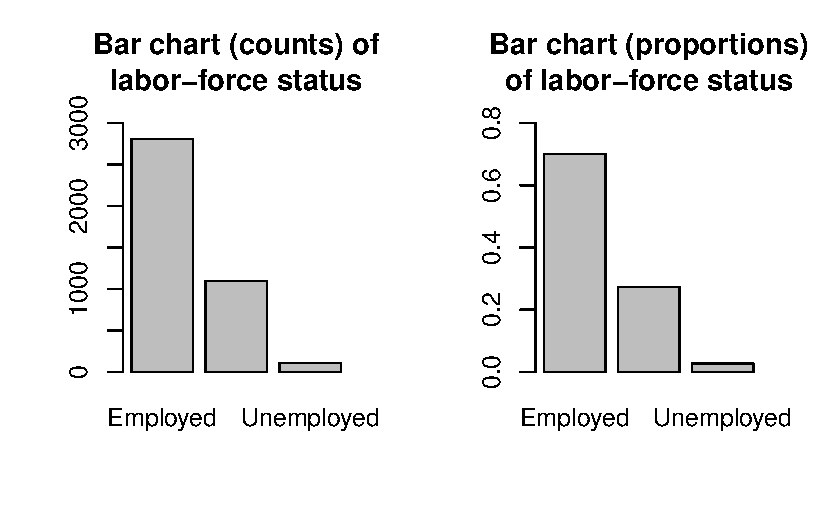
\includegraphics[keepaspectratio]{lab-03_files/figure-pdf/cps bar chart-1.pdf}}

\subsubsection{Numerical Data: Example}\label{numerical-data-example}

\emph{Histogram of 2019 CPS age distribution}
\AddToHookNext{env/Highlighting/begin}{\small}

\pandocbounded{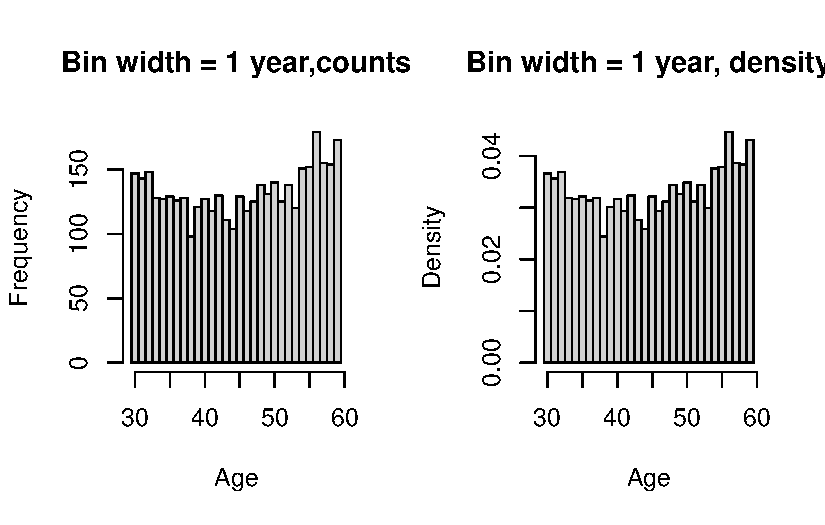
\includegraphics[keepaspectratio]{lab-03_files/figure-pdf/cps histogram-1.pdf}}

\emph{Histogram and density plot of 2019 CPS weekly earnings
distribution of employed individuals}
\AddToHookNext{env/Highlighting/begin}{\small}

\pandocbounded{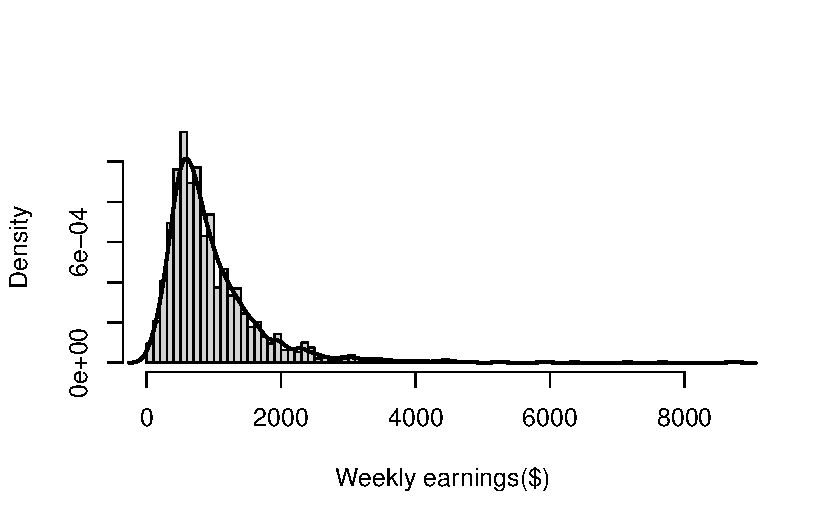
\includegraphics[keepaspectratio]{lab-03_files/figure-pdf/cps histogram and density-1.pdf}}

\subsubsection{Sample quantiles:
Example}\label{sample-quantiles-example}

\emph{Sample quantiles of 2019 CPS weekly earnings quantiles}
\AddToHookNext{env/Highlighting/begin}{\small}

\begin{Shaded}
\begin{Highlighting}[]
\CommentTok{\# Histogram with density}
\FunctionTok{hist}\NormalTok{(cpsemployed}\SpecialCharTok{$}\NormalTok{earnwk, }\AttributeTok{breaks=}\DecValTok{92}\NormalTok{, }\AttributeTok{freq=}\ConstantTok{FALSE}\NormalTok{,}
     \AttributeTok{main=}\StringTok{""}\NormalTok{, }\AttributeTok{xlab=}\StringTok{"Weekly earnings($)"}\NormalTok{)}
\FunctionTok{lines}\NormalTok{(}\FunctionTok{density}\NormalTok{(cpsemployed}\SpecialCharTok{$}\NormalTok{earnwk), }\AttributeTok{lwd=}\DecValTok{2}\NormalTok{, }\AttributeTok{lty=}\DecValTok{1}\NormalTok{)}

\CommentTok{\# Quantiles}
\NormalTok{qs }\OtherTok{\textless{}{-}} \FunctionTok{quantile}\NormalTok{(cpsemployed}\SpecialCharTok{$}\NormalTok{earnwk, }\AttributeTok{probs=}\FunctionTok{c}\NormalTok{(}\FloatTok{0.05}\NormalTok{, }\FloatTok{0.10}\NormalTok{, }\FloatTok{0.25}\NormalTok{, }
                                           \FloatTok{0.50}\NormalTok{, }\FloatTok{0.75}\NormalTok{, }\FloatTok{0.90}\NormalTok{, }\FloatTok{0.95}\NormalTok{),}
               \AttributeTok{na.rm=}\ConstantTok{TRUE}\NormalTok{)}

\CommentTok{\# Brewer palette with 7 distinct colors}
\NormalTok{cols }\OtherTok{\textless{}{-}} \FunctionTok{brewer.pal}\NormalTok{(}\AttributeTok{n=}\DecValTok{7}\NormalTok{, }\AttributeTok{name=}\StringTok{"Set1"}\NormalTok{)}

\CommentTok{\# Add vertical lines with colors}
\ControlFlowTok{for}\NormalTok{ (i }\ControlFlowTok{in} \FunctionTok{seq\_along}\NormalTok{(qs)) \{}
  \FunctionTok{abline}\NormalTok{(}\AttributeTok{v=}\NormalTok{qs[i], }\AttributeTok{col=}\NormalTok{cols[i], }\AttributeTok{lwd=}\DecValTok{2}\NormalTok{, }\AttributeTok{lty=}\DecValTok{2}\NormalTok{)}
\NormalTok{\}}

\CommentTok{\# Legend}
\FunctionTok{legend}\NormalTok{(}\StringTok{"topright"}\NormalTok{, }\AttributeTok{legend=}\FunctionTok{names}\NormalTok{(qs),}
       \AttributeTok{col=}\NormalTok{cols, }\AttributeTok{lwd=}\DecValTok{2}\NormalTok{, }\AttributeTok{lty=}\DecValTok{1}\NormalTok{, }\AttributeTok{cex=}\FloatTok{0.8}\NormalTok{,}
       \AttributeTok{title=}\StringTok{"Quantiles"}\NormalTok{)}
\end{Highlighting}
\end{Shaded}

\pandocbounded{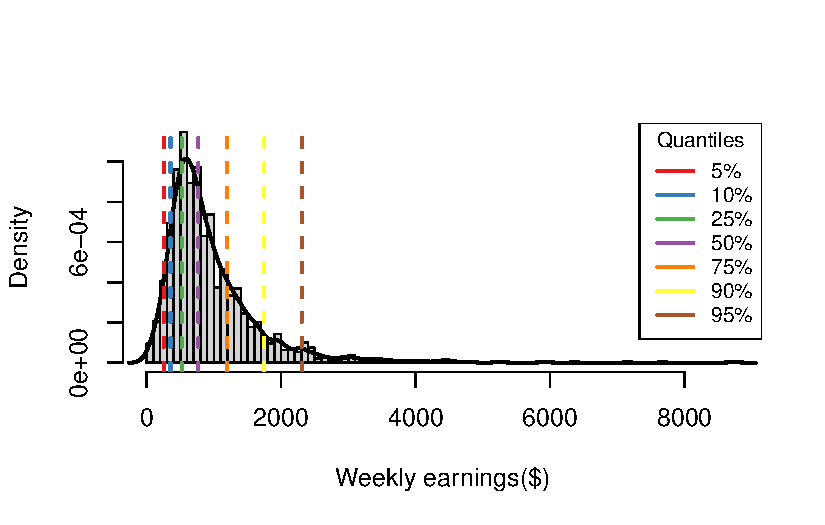
\includegraphics[keepaspectratio]{lab-03_files/figure-pdf/cps sample quantiles-1.pdf}}

\subsubsection{Boxplot: Example}\label{boxplot-example}

\emph{2019 CPS weekly earnings}
\AddToHookNext{env/Highlighting/begin}{\small}

\begin{Shaded}
\begin{Highlighting}[]
\FunctionTok{par}\NormalTok{(}\AttributeTok{mfrow =} \FunctionTok{c}\NormalTok{(}\DecValTok{1}\NormalTok{,}\DecValTok{2}\NormalTok{), }\AttributeTok{pin=}\FunctionTok{c}\NormalTok{(}\DecValTok{2}\NormalTok{,}\DecValTok{3}\NormalTok{))}
\CommentTok{\# box plot with whiskers and outliers (the default in R)}
\FunctionTok{boxplot}\NormalTok{(cpsemployed}\SpecialCharTok{$}\NormalTok{earnwk, }\AttributeTok{ylab=}\StringTok{"Weekly earnings"}\NormalTok{,}
\AttributeTok{main=}\StringTok{"Box plot (whiskers and outliers)"}\NormalTok{)}
\CommentTok{\# box plot with whiskers at min and max values}
\FunctionTok{boxplot}\NormalTok{(cpsemployed}\SpecialCharTok{$}\NormalTok{earnwk, }\AttributeTok{range=}\DecValTok{0}\NormalTok{,}\AttributeTok{ylab=}\StringTok{"Weekly earnings"}\NormalTok{,}
\AttributeTok{main=}\StringTok{"Box plot (whiskers at min/max)"}\NormalTok{)}
\end{Highlighting}
\end{Shaded}

\pandocbounded{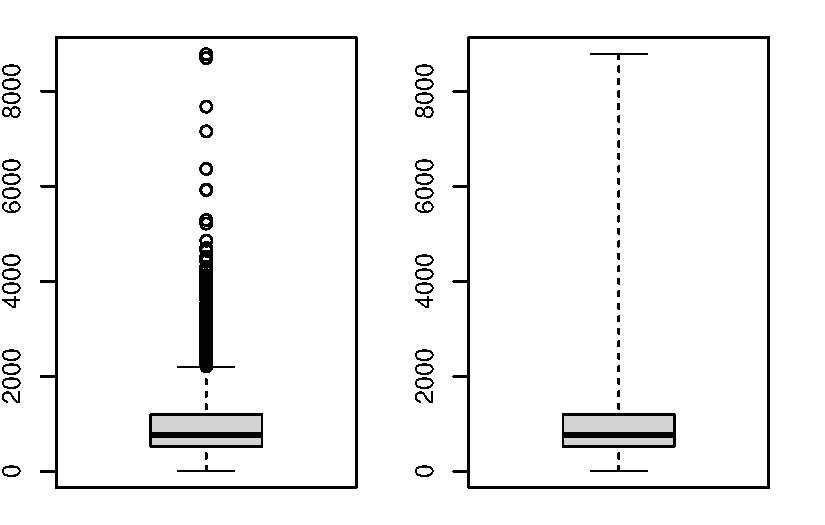
\includegraphics[keepaspectratio]{lab-03_files/figure-pdf/cps boxplot-1.pdf}}

\subsubsection{Descriptive statistics:
Example}\label{descriptive-statistics-example}

\emph{2019 CPS Union vs Non-union worker's wage}
\AddToHookNext{env/Highlighting/begin}{\small}

\begin{Shaded}
\begin{Highlighting}[]
\NormalTok{union\_summary}\OtherTok{\textless{}{-}}\NormalTok{cpsemployed}\SpecialCharTok{\%\textgreater{}\%}
  \FunctionTok{group\_by}\NormalTok{(unionstatus)}\SpecialCharTok{\%\textgreater{}\%}
  \FunctionTok{summarise}\NormalTok{(}
    \AttributeTok{n =} \FunctionTok{n}\NormalTok{(),}
    \AttributeTok{mean =} \FunctionTok{round}\NormalTok{(}\FunctionTok{mean}\NormalTok{(earnwk, }\AttributeTok{na.rm =} \ConstantTok{TRUE}\NormalTok{),}\DecValTok{2}\NormalTok{),}
    \AttributeTok{MAD =} \FunctionTok{round}\NormalTok{(}\FunctionTok{mean}\NormalTok{(}\FunctionTok{abs}\NormalTok{(earnwk }\SpecialCharTok{{-}} \FunctionTok{mean}\NormalTok{(earnwk, }\AttributeTok{na.rm =} \ConstantTok{TRUE}\NormalTok{)), }\AttributeTok{na.rm =} \ConstantTok{TRUE}\NormalTok{),}\DecValTok{2}\NormalTok{),}
    \AttributeTok{variance =} \FunctionTok{round}\NormalTok{(}\FunctionTok{var}\NormalTok{(earnwk, }\AttributeTok{na.rm =} \ConstantTok{TRUE}\NormalTok{),}\DecValTok{2}\NormalTok{),   }\CommentTok{\# uses n{-}1 in denominator}
    \AttributeTok{sd =} \FunctionTok{round}\NormalTok{(}\FunctionTok{sd}\NormalTok{(earnwk, }\AttributeTok{na.rm =} \ConstantTok{TRUE}\NormalTok{),}\DecValTok{2}\NormalTok{)}
\NormalTok{  )}
\NormalTok{union\_summary}
\end{Highlighting}
\end{Shaded}

\begin{verbatim}
# A tibble: 2 x 6
  unionstatus     n  mean   MAD variance    sd
  <fct>       <int> <dbl> <dbl>    <dbl> <dbl>
1 Non-union    2533  946.  489.  562120.  750.
2 Union         276 1198.  532.  518379.  720.
\end{verbatim}

\begin{Shaded}
\begin{Highlighting}[]
\FunctionTok{kbl}\NormalTok{(union\_summary, }\AttributeTok{format=}\StringTok{"latex"}\NormalTok{, }\AttributeTok{booktabs =}\NormalTok{ T, }\AttributeTok{escape=}\NormalTok{F,}
    \AttributeTok{align=}\FunctionTok{c}\NormalTok{(}\StringTok{"l"}\NormalTok{,}\StringTok{"c"}\NormalTok{,}\StringTok{"c"}\NormalTok{,}\StringTok{"c"}\NormalTok{,}\StringTok{"c"}\NormalTok{,}\StringTok{"c"}\NormalTok{),}
    \AttributeTok{caption =} \StringTok{"Union vs non{-}union worker\textquotesingle{}s wage (CPS, 2019)"}\NormalTok{,}
    \AttributeTok{col.names =} \FunctionTok{c}\NormalTok{(}\StringTok{"Union Status"}\NormalTok{, }\StringTok{"Sample Size ($n$)"}\NormalTok{, }\StringTok{"Mean ($}\SpecialCharTok{\textbackslash{}\textbackslash{}}\StringTok{overline\{x\}$)"}\NormalTok{, }
                  \StringTok{"MAD"}\NormalTok{, }\StringTok{"Variance ($s\_x\^{}2$)"}\NormalTok{, }\StringTok{"Std. Dev. ($s\_x$)"}\NormalTok{)) }\SpecialCharTok{\%\textgreater{}\%}
  \FunctionTok{kable\_styling}\NormalTok{(}\AttributeTok{position =} \StringTok{"center"}\NormalTok{)}\SpecialCharTok{\%\textgreater{}\%}
\FunctionTok{footnote}\NormalTok{(}\AttributeTok{general =} \StringTok{"Here is a general notes for this table."}\NormalTok{)}
\end{Highlighting}
\end{Shaded}

\begin{table}
\centering
\caption{\label{tab:cps desc 1}Union vs non-union worker's wage (CPS, 2019)}
\centering
\begin{tabular}[t]{lccccc}
\toprule
Union Status & Sample Size ($n$) & Mean ($\overline{x}$) & MAD & Variance ($s_x^2$) & Std. Dev. ($s_x$)\\
\midrule
Non-union & 2533 & 946.50 & 488.79 & 562120.3 & 749.75\\
Union & 276 & 1197.65 & 532.42 & 518378.8 & 719.99\\
\bottomrule
\multicolumn{6}{l}{\rule{0pt}{1em}\textit{Note: }}\\
\multicolumn{6}{l}{\rule{0pt}{1em}Here is a general notes for this table.}\\
\end{tabular}
\end{table}

\emph{2019 CPS Male vs female worker's wage}
\AddToHookNext{env/Highlighting/begin}{\small}

\begin{Shaded}
\begin{Highlighting}[]
\NormalTok{gender\_summary}\OtherTok{\textless{}{-}}\NormalTok{cpsemployed}\SpecialCharTok{\%\textgreater{}\%}
  \FunctionTok{group\_by}\NormalTok{(gender)}\SpecialCharTok{\%\textgreater{}\%}
  \FunctionTok{summarise}\NormalTok{(}
     \AttributeTok{n =} \FunctionTok{n}\NormalTok{(),}
    \AttributeTok{mean =} \FunctionTok{round}\NormalTok{(}\FunctionTok{mean}\NormalTok{(earnwk, }\AttributeTok{na.rm =} \ConstantTok{TRUE}\NormalTok{),}\DecValTok{2}\NormalTok{),}
    \AttributeTok{MAD =} \FunctionTok{round}\NormalTok{(}\FunctionTok{mean}\NormalTok{(}\FunctionTok{abs}\NormalTok{(earnwk }\SpecialCharTok{{-}} \FunctionTok{mean}\NormalTok{(earnwk, }\AttributeTok{na.rm =} \ConstantTok{TRUE}\NormalTok{)), }\AttributeTok{na.rm =} \ConstantTok{TRUE}\NormalTok{),}\DecValTok{2}\NormalTok{),}
    \AttributeTok{variance =} \FunctionTok{round}\NormalTok{(}\FunctionTok{var}\NormalTok{(earnwk, }\AttributeTok{na.rm =} \ConstantTok{TRUE}\NormalTok{),}\DecValTok{2}\NormalTok{),   }\CommentTok{\# uses n{-}1 in denominator}
    \AttributeTok{sd =} \FunctionTok{round}\NormalTok{(}\FunctionTok{sd}\NormalTok{(earnwk, }\AttributeTok{na.rm =} \ConstantTok{TRUE}\NormalTok{),}\DecValTok{2}\NormalTok{)}
\NormalTok{  )}
\NormalTok{gender\_summary}
\end{Highlighting}
\end{Shaded}

\begin{verbatim}
# A tibble: 2 x 6
  gender     n  mean   MAD variance    sd
  <fct>  <int> <dbl> <dbl>    <dbl> <dbl>
1 Female  1308  803.  415.  457066.  676.
2 Male    1501 1117.  530.  610218.  781.
\end{verbatim}

\begin{Shaded}
\begin{Highlighting}[]
\FunctionTok{kbl}\NormalTok{(gender\_summary,}\AttributeTok{format=}\StringTok{"latex"}\NormalTok{, }\AttributeTok{booktabs =}\NormalTok{ T, }\AttributeTok{escape=}\NormalTok{F,}
    \AttributeTok{align=}\FunctionTok{c}\NormalTok{(}\StringTok{"l"}\NormalTok{,}\StringTok{"c"}\NormalTok{,}\StringTok{"c"}\NormalTok{,}\StringTok{"c"}\NormalTok{,}\StringTok{"c"}\NormalTok{,}\StringTok{"c"}\NormalTok{),}
    \AttributeTok{caption =} \StringTok{"Male vs female worker\textquotesingle{}s wage (CPS, 2019)"}\NormalTok{,}
    \AttributeTok{col.names =} \FunctionTok{c}\NormalTok{(}\StringTok{"Gender"}\NormalTok{, }\StringTok{"Sample Size ($n$)"}\NormalTok{, }\StringTok{"Mean ($}\SpecialCharTok{\textbackslash{}\textbackslash{}}\StringTok{overline\{x\}$)"}\NormalTok{, }
                  \StringTok{"MAD"}\NormalTok{, }\StringTok{"Variance ($s\_x\^{}2$)"}\NormalTok{, }\StringTok{"Std. Dev. ($s\_x$)"}\NormalTok{)) }\SpecialCharTok{\%\textgreater{}\%}
  \FunctionTok{kable\_styling}\NormalTok{(}\AttributeTok{position =} \StringTok{"center"}\NormalTok{)}
\end{Highlighting}
\end{Shaded}

\begin{table}
\centering
\caption{\label{tab:cps desc 2}Male vs female worker's wage (CPS, 2019)}
\centering
\begin{tabular}[t]{lccccc}
\toprule
Gender & Sample Size ($n$) & Mean ($\overline{x}$) & MAD & Variance ($s_x^2$) & Std. Dev. ($s_x$)\\
\midrule
Female & 1308 & 803.49 & 415.14 & 457066.4 & 676.07\\
Male & 1501 & 1117.30 & 529.94 & 610217.8 & 781.16\\
\bottomrule
\end{tabular}
\end{table}

\subsection{Multiple variable}\label{multiple-variable}

\subsubsection{Joint sample counts or proportion:
Example}\label{joint-sample-counts-or-proportion-example}

\textbf{Joint sample count for labor-force status and race}

\begin{Shaded}
\begin{Highlighting}[]
\NormalTok{joint\_count}\OtherTok{\textless{}{-}}\FunctionTok{addmargins}\NormalTok{(}\FunctionTok{table}\NormalTok{(cps}\SpecialCharTok{$}\NormalTok{lfstatus, cps}\SpecialCharTok{$}\NormalTok{race))}
\FunctionTok{kbl}\NormalTok{(joint\_count, }\AttributeTok{booktabs =}\NormalTok{ T) }\SpecialCharTok{\%\textgreater{}\%}
  \FunctionTok{kable\_styling}\NormalTok{(}\AttributeTok{position =} \StringTok{"center"}\NormalTok{)}
\end{Highlighting}
\end{Shaded}

\begin{table}
\centering
\begin{tabular}[t]{lrrrr}
\toprule
  & Black & Other & White & Sum\\
\midrule
Employed & 324 & 241 & 2244 & 2809\\
Not in LF & 136 & 99 & 863 & 1098\\
Unemployed & 16 & 9 & 81 & 106\\
Sum & 476 & 349 & 3188 & 4013\\
\bottomrule
\end{tabular}
\end{table}

\textbf{Joint sample proportion for labor-force status and race}

\begin{Shaded}
\begin{Highlighting}[]
\NormalTok{joint\_proportion}\OtherTok{\textless{}{-}}\FunctionTok{round}\NormalTok{(}\FunctionTok{addmargins}\NormalTok{(}\FunctionTok{table}\NormalTok{(cps}\SpecialCharTok{$}\NormalTok{lfstatus, cps}\SpecialCharTok{$}\NormalTok{race))}\SpecialCharTok{/}\FunctionTok{nrow}\NormalTok{(cps),}\DecValTok{3}\NormalTok{)}
\FunctionTok{kbl}\NormalTok{(joint\_proportion, }\AttributeTok{booktabs =}\NormalTok{ T) }\SpecialCharTok{\%\textgreater{}\%}
  \FunctionTok{kable\_styling}\NormalTok{(}\AttributeTok{position =} \StringTok{"center"}\NormalTok{)}
\end{Highlighting}
\end{Shaded}

\begin{table}
\centering
\begin{tabular}[t]{lrrrr}
\toprule
  & Black & Other & White & Sum\\
\midrule
Employed & 0.081 & 0.060 & 0.559 & 0.700\\
Not in LF & 0.034 & 0.025 & 0.215 & 0.274\\
Unemployed & 0.004 & 0.002 & 0.020 & 0.026\\
Sum & 0.119 & 0.087 & 0.794 & 1.000\\
\bottomrule
\end{tabular}
\end{table}

\textbf{Sample proportions of labor-force status conditional on race}

\begin{Shaded}
\begin{Highlighting}[]
\NormalTok{joint\_proportion\_race}\OtherTok{\textless{}{-}}\FunctionTok{round}\NormalTok{(}\FunctionTok{prop.table}\NormalTok{(}\FunctionTok{table}\NormalTok{(cps}\SpecialCharTok{$}\NormalTok{lfstatus, cps}\SpecialCharTok{$}\NormalTok{race),}\AttributeTok{margin=}\DecValTok{2}\NormalTok{),}\DecValTok{3}\NormalTok{)}
\FunctionTok{kbl}\NormalTok{(joint\_proportion\_race, }\AttributeTok{booktabs =}\NormalTok{ T) }\SpecialCharTok{\%\textgreater{}\%}
  \FunctionTok{kable\_styling}\NormalTok{(}\AttributeTok{position =} \StringTok{"center"}\NormalTok{)}
\end{Highlighting}
\end{Shaded}

\begin{table}
\centering
\begin{tabular}[t]{lrrr}
\toprule
  & Black & Other & White\\
\midrule
Employed & 0.681 & 0.691 & 0.704\\
Not in LF & 0.286 & 0.284 & 0.271\\
Unemployed & 0.034 & 0.026 & 0.025\\
\bottomrule
\end{tabular}
\end{table}

\textbf{Sample proportions of race conditional on labor-force status}

\begin{Shaded}
\begin{Highlighting}[]
\NormalTok{joint\_proportion\_lfstatus}\OtherTok{\textless{}{-}}\FunctionTok{round}\NormalTok{(}\FunctionTok{prop.table}\NormalTok{(}\FunctionTok{table}\NormalTok{(cps}\SpecialCharTok{$}\NormalTok{lfstatus, cps}\SpecialCharTok{$}\NormalTok{race),}\AttributeTok{margin=}\DecValTok{1}\NormalTok{),}\DecValTok{3}\NormalTok{)}
\FunctionTok{kbl}\NormalTok{(joint\_proportion\_lfstatus, }\AttributeTok{booktabs =}\NormalTok{ T) }\SpecialCharTok{\%\textgreater{}\%}
  \FunctionTok{kable\_styling}\NormalTok{(}\AttributeTok{position =} \StringTok{"center"}\NormalTok{)}
\end{Highlighting}
\end{Shaded}

\begin{table}
\centering
\begin{tabular}[t]{lrrr}
\toprule
  & Black & Other & White\\
\midrule
Employed & 0.115 & 0.086 & 0.799\\
Not in LF & 0.124 & 0.090 & 0.786\\
Unemployed & 0.151 & 0.085 & 0.764\\
\bottomrule
\end{tabular}
\end{table}

\subsubsection{Bar charts: Example}\label{bar-charts-example}

\textbf{Labor-force status proportions by race}

\begin{Shaded}
\begin{Highlighting}[]
\CommentTok{\# create sample count table for race and labor{-}force status variables}
\NormalTok{tbl\_racelf }\OtherTok{\textless{}{-}} \FunctionTok{table}\NormalTok{(cps}\SpecialCharTok{$}\NormalTok{race, cps}\SpecialCharTok{$}\NormalTok{lfstatus)}
\CommentTok{\# barplot command {-}{-}{-} categories on x{-}axis are based upon columns (lfstatus) of the table}
\FunctionTok{barplot}\NormalTok{(}\FunctionTok{prop.table}\NormalTok{(tbl\_racelf, }\AttributeTok{margin=}\DecValTok{1}\NormalTok{), }\AttributeTok{ylim=}\FunctionTok{c}\NormalTok{(}\DecValTok{0}\NormalTok{,}\FloatTok{0.8}\NormalTok{), }\AttributeTok{col=}\FunctionTok{c}\NormalTok{(}\StringTok{"gray30"}\NormalTok{,}\StringTok{"gray50"}\NormalTok{, }\StringTok{"gray70"}\NormalTok{),}
\AttributeTok{legend.text=}\FunctionTok{rownames}\NormalTok{(tbl\_racelf), }\AttributeTok{beside=}\ConstantTok{TRUE}\NormalTok{, }\AttributeTok{main=}\StringTok{""}\NormalTok{)}
\end{Highlighting}
\end{Shaded}

\pandocbounded{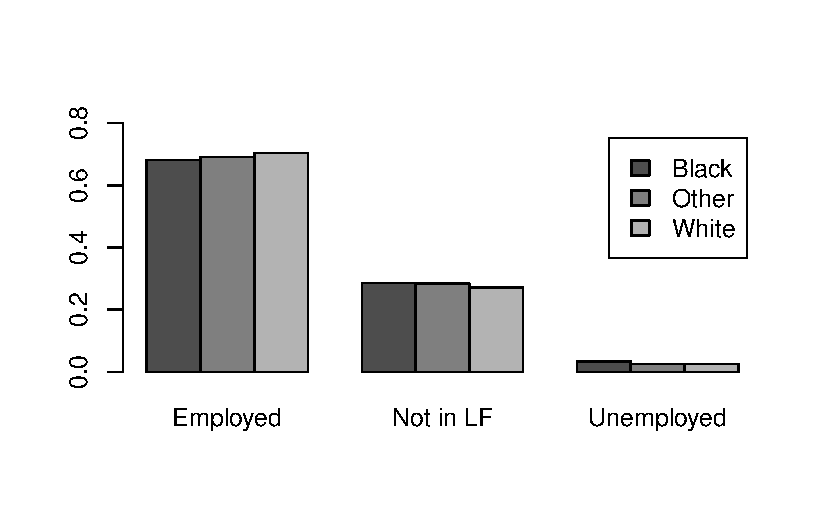
\includegraphics[keepaspectratio]{lab-03_files/figure-pdf/cps bar chart by race-1.pdf}}

\textbf{Race proportions by labor-force status* \{.smaller
auto-animate=``true''\}}

\begin{Shaded}
\begin{Highlighting}[]
\CommentTok{\# create sample count table table for race and labor{-}force status variables}
\NormalTok{tbl\_lfrace }\OtherTok{\textless{}{-}} \FunctionTok{table}\NormalTok{(cps}\SpecialCharTok{$}\NormalTok{lfstatus, cps}\SpecialCharTok{$}\NormalTok{race)}
\CommentTok{\# barplot command {-}{-}{-} categories on x{-}axis are based upon columns (race) of the table}
\FunctionTok{barplot}\NormalTok{(}\FunctionTok{prop.table}\NormalTok{(tbl\_lfrace, }\AttributeTok{margin=}\DecValTok{1}\NormalTok{), }\AttributeTok{ylim=}\FunctionTok{c}\NormalTok{(}\DecValTok{0}\NormalTok{,}\FloatTok{0.8}\NormalTok{), }\AttributeTok{col=}\FunctionTok{c}\NormalTok{(}\StringTok{"gray30"}\NormalTok{,}\StringTok{"gray50"}\NormalTok{, }\StringTok{"gray70"}\NormalTok{),}
\AttributeTok{legend.text=}\FunctionTok{rownames}\NormalTok{(tbl\_lfrace), }\AttributeTok{beside=}\ConstantTok{TRUE}\NormalTok{,}
\AttributeTok{args.legend =} \FunctionTok{list}\NormalTok{(}\AttributeTok{x=}\StringTok{"topleft"}\NormalTok{,}\AttributeTok{inset=}\FloatTok{0.01}\NormalTok{), }\AttributeTok{main=}\StringTok{""}\NormalTok{)}
\end{Highlighting}
\end{Shaded}

\pandocbounded{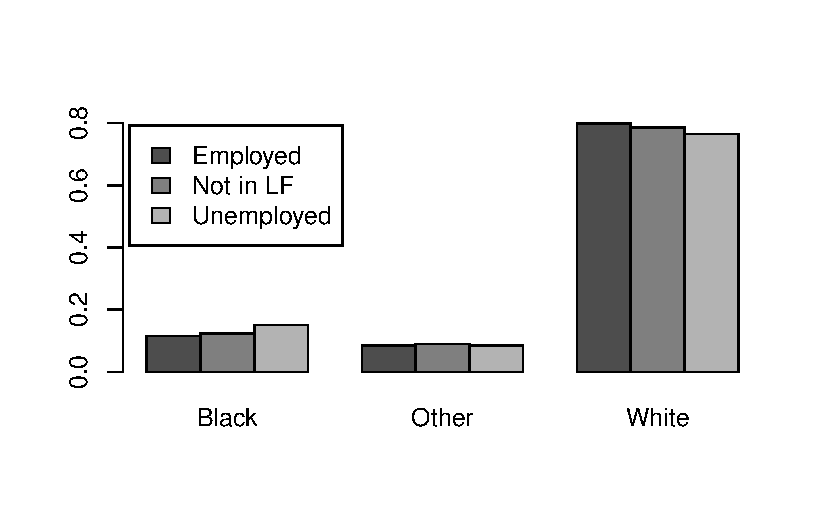
\includegraphics[keepaspectratio]{lab-03_files/figure-pdf/cps bar chart by lfstatus-1.pdf}}

\subsubsection{Showing distribution for different category:
Example}\label{showing-distribution-for-different-category-example}

\textbf{Box plots of weekly earnings by race}

\begin{Shaded}
\begin{Highlighting}[]
\FunctionTok{boxplot}\NormalTok{(cps}\SpecialCharTok{$}\NormalTok{earnwk}\SpecialCharTok{\textasciitilde{}}\NormalTok{cps}\SpecialCharTok{$}\NormalTok{race, }\AttributeTok{ylab=}\StringTok{"Weekly earnings ($)"}\NormalTok{, }\AttributeTok{xlab=}\StringTok{"Race"}\NormalTok{)}
\end{Highlighting}
\end{Shaded}

\pandocbounded{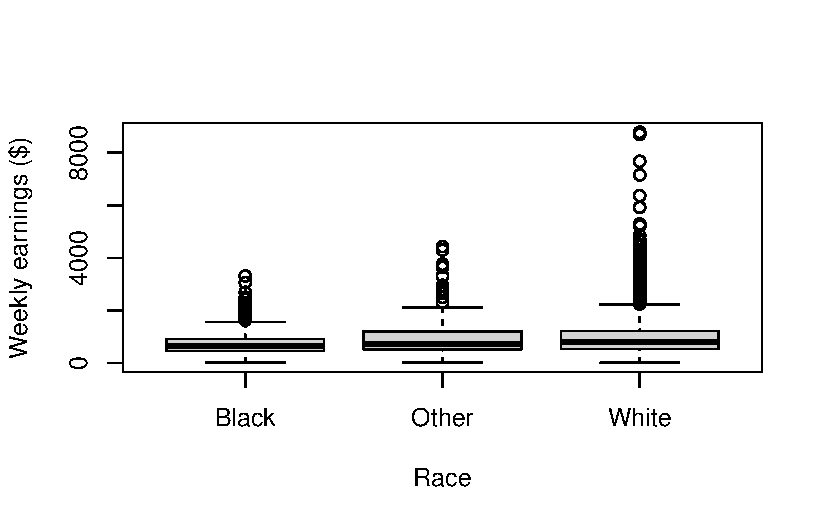
\includegraphics[keepaspectratio]{lab-03_files/figure-pdf/box plot earnings race-1.pdf}}

\textbf{Density of weakly earnings by race}

\begin{Shaded}
\begin{Highlighting}[]
\CommentTok{\# createweeklyearningsvectorsforthethreesubsamples,byrace}
\NormalTok{earnwk\_black }\OtherTok{\textless{}{-}}\NormalTok{cpsemployed[cpsemployed}\SpecialCharTok{$}\NormalTok{race}\SpecialCharTok{==}\StringTok{"Black"}\NormalTok{,}\StringTok{"earnwk"}\NormalTok{]}
\NormalTok{earnwk\_other }\OtherTok{\textless{}{-}}\NormalTok{cpsemployed[cpsemployed}\SpecialCharTok{$}\NormalTok{race}\SpecialCharTok{==}\StringTok{"Other"}\NormalTok{,}\StringTok{"earnwk"}\NormalTok{]}
\NormalTok{earnwk\_white }\OtherTok{\textless{}{-}}\NormalTok{cpsemployed[cpsemployed}\SpecialCharTok{$}\NormalTok{race}\SpecialCharTok{==}\StringTok{"White"}\NormalTok{,}\StringTok{"earnwk"}\NormalTok{]}
\CommentTok{\# firstplotthedensityofweeklyearningsforblackindividuals}
\FunctionTok{plot}\NormalTok{(}\FunctionTok{density}\NormalTok{(earnwk\_black), }\AttributeTok{main=}\StringTok{""}\NormalTok{,}\AttributeTok{xlab=}\StringTok{"Weekly earnings($)"}\NormalTok{)}
\CommentTok{\# overlaythedensityofweeklyearningsforother{-}raceindividuals}
\FunctionTok{lines}\NormalTok{(}\FunctionTok{density}\NormalTok{(earnwk\_other), }\AttributeTok{lty=}\DecValTok{3}\NormalTok{)}
\CommentTok{\# overlaythedensityofweeklyearningsforwhiteindividuals}
\FunctionTok{lines}\NormalTok{(}\FunctionTok{density}\NormalTok{(earnwk\_white), }\AttributeTok{lty=}\DecValTok{2}\NormalTok{)}
\CommentTok{\# drawthelegend}
\FunctionTok{legend}\NormalTok{(}\StringTok{"topright"}\NormalTok{, }\AttributeTok{legend=}\FunctionTok{c}\NormalTok{(}\StringTok{"Black"}\NormalTok{,}\StringTok{"Other"}\NormalTok{,}\StringTok{"White"}\NormalTok{), }\AttributeTok{lty=}\FunctionTok{c}\NormalTok{(}\DecValTok{1}\NormalTok{,}\DecValTok{3}\NormalTok{,}\DecValTok{2}\NormalTok{), }\AttributeTok{inset=}\FloatTok{0.01}\NormalTok{)}
\end{Highlighting}
\end{Shaded}

\pandocbounded{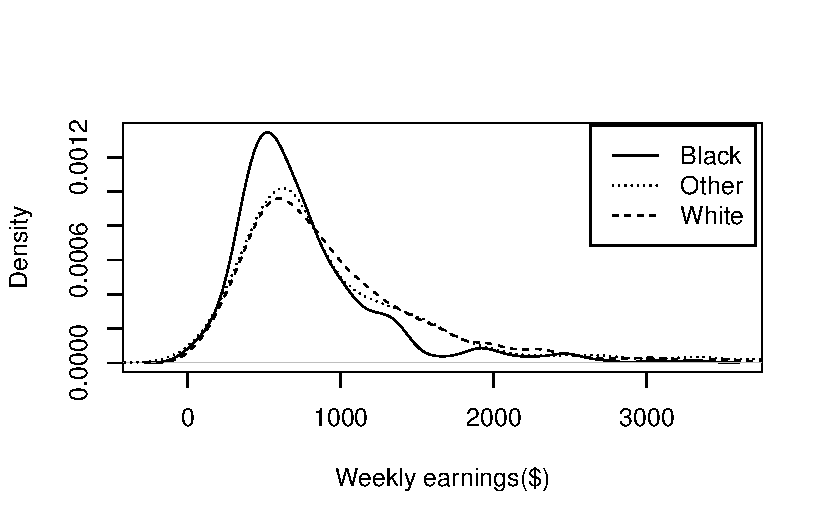
\includegraphics[keepaspectratio]{lab-03_files/figure-pdf/density earnings race-1.pdf}}

\subsubsection{Scatterplot: Example}\label{scatterplot-example}

\textbf{Weekly earnings versus years of education}

\begin{Shaded}
\begin{Highlighting}[]
\CommentTok{\# scatterplotofweeklyearningsversusyearsofeducation}
\FunctionTok{plot}\NormalTok{(cps}\SpecialCharTok{$}\NormalTok{educ, cps}\SpecialCharTok{$}\NormalTok{earnwk,}\AttributeTok{xlab=}\StringTok{"Education"}\NormalTok{,}\AttributeTok{ylab=}\StringTok{"Weekly earnings($)"}\NormalTok{)}
\end{Highlighting}
\end{Shaded}

\pandocbounded{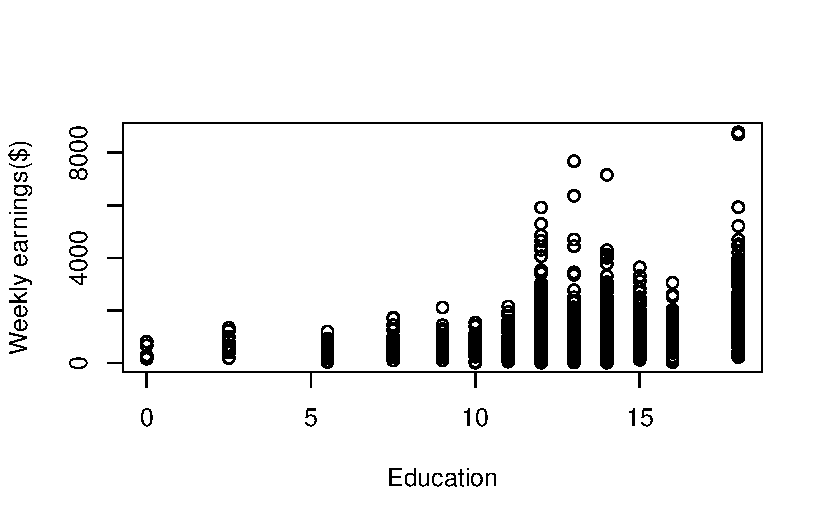
\includegraphics[keepaspectratio]{lab-03_files/figure-pdf/scatter earnings years-1.pdf}}

\subsubsection{Expanded scatterplot:
Example}\label{expanded-scatterplot-example}

\textbf{Weekly earnings vs years of education vs weekly hours worked}

\begin{Shaded}
\begin{Highlighting}[]
\CommentTok{\# expandedscatterplot,withweeklyearnings,yearsofeducation,andweeklyhoursworked}
\FunctionTok{plot}\NormalTok{(cps[,}\FunctionTok{c}\NormalTok{(}\StringTok{"educ"}\NormalTok{,}\StringTok{"earnwk"}\NormalTok{,}\StringTok{"hrslastwk"}\NormalTok{)])}
\end{Highlighting}
\end{Shaded}

\pandocbounded{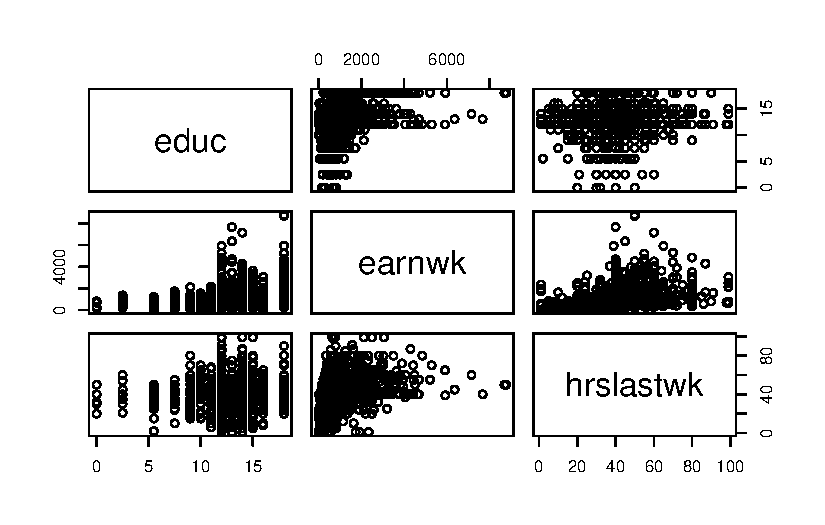
\includegraphics[keepaspectratio]{lab-03_files/figure-pdf/expanded scatter-1.pdf}}

\section{Exercise 4: Performing better data
visualization}\label{exercise-4-performing-better-data-visualization}

There is website that host a collection of beautiful charts you might
want to visit: \texttt{https://r-graph-gallery.com/}. This exercise will
require you to use the \texttt{cps} data we used above or other datasets
from the textbooks package (see at
\texttt{https://probstats4econ.com/datasets.html}), then produce the
data visualization by replicating the code you find in the websites.
Choose two graph that you really like and try to replicate it in the
following code chunks. Remember to install the packages needed to
produce the graph by putting the package name in the
\texttt{package\ manager} chunk.

\emph{Visualization replication 1}
\AddToHookNext{env/Highlighting/begin}{\small}

\begin{Shaded}
\begin{Highlighting}[]
\FunctionTok{plot}\NormalTok{(cps[, }\FunctionTok{c}\NormalTok{(}\StringTok{"lfstatus"}\NormalTok{, }\StringTok{"age"}\NormalTok{)])}
\end{Highlighting}
\end{Shaded}

\pandocbounded{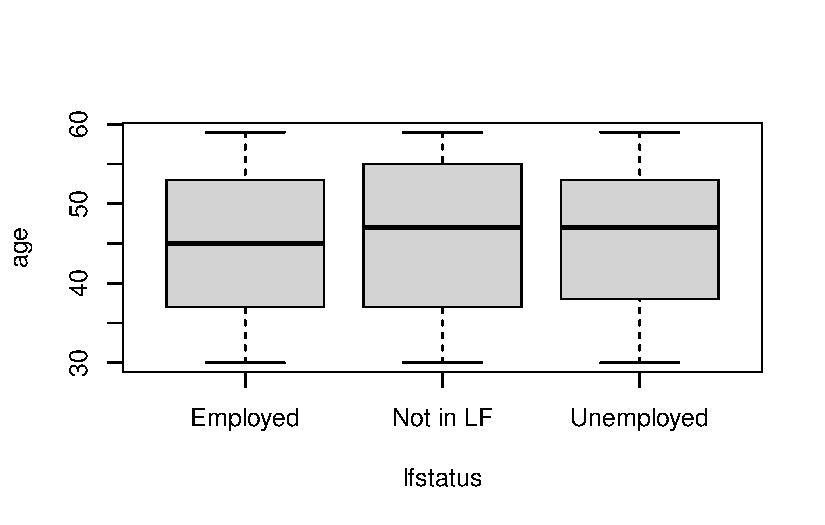
\includegraphics[keepaspectratio]{lab-03_files/figure-pdf/r graph gallery replication 1-1.pdf}}

\emph{Visualization replication 2}
\AddToHookNext{env/Highlighting/begin}{\small}

\begin{Shaded}
\begin{Highlighting}[]
\CommentTok{\# Load ggplot2}
\FunctionTok{library}\NormalTok{(ggplot2)}

\CommentTok{\# Create data}
\NormalTok{data }\OtherTok{\textless{}{-}} \FunctionTok{data.frame}\NormalTok{(}
\NormalTok{  cps}
\NormalTok{  )}

\CommentTok{\# Barplot}
\FunctionTok{ggplot}\NormalTok{(data, }\FunctionTok{aes}\NormalTok{(}\AttributeTok{x=}\NormalTok{lfstatus, }\AttributeTok{y=}\NormalTok{ownchild)) }\SpecialCharTok{+} 
  \FunctionTok{geom\_bar}\NormalTok{(}\AttributeTok{stat =} \StringTok{"identity"}\NormalTok{)}
\end{Highlighting}
\end{Shaded}

\pandocbounded{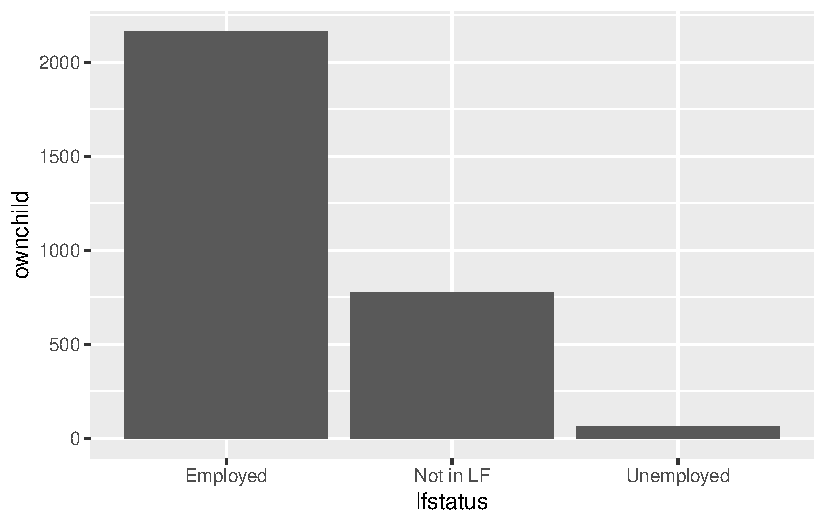
\includegraphics[keepaspectratio]{lab-03_files/figure-pdf/r graph gallery replication 2-1.pdf}}

\section{Wrapping up}\label{wrapping-up}

\textbf{Team Member 1}: Render the document and confirm that the changes
are visible in the PDF. Then, commit (with an informative commit
message) both the .qmd and PDF documents, and finally push the changes
to GitHub. Make sure to commit and push all changed files so that your
Git pane is empty afterwards.

\textbf{All other team members}: Once Team Member 2 is done rendering,
committing, and pushing, confirm that the changes are visible on GitHub
in your team's lab repo. Then, in RStudio, click the Pull button in the
Git pane to get the updated document. You should see the final version
of your .qmd file.

\section{Submission}\label{submission}

You will submit the PDF documents for labs in to Gradescope as part of
your final submission.

\begin{tcolorbox}[enhanced jigsaw, leftrule=.75mm, bottomtitle=1mm, breakable, colback=white, toprule=.15mm, toptitle=1mm, left=2mm, colbacktitle=quarto-callout-warning-color!10!white, colframe=quarto-callout-warning-color-frame, opacitybacktitle=0.6, titlerule=0mm, coltitle=black, opacityback=0, title=\textcolor{quarto-callout-warning-color}{\faExclamationTriangle}\hspace{0.5em}{Warning}, arc=.35mm, rightrule=.15mm, bottomrule=.15mm]

Before you wrap up the assignment, make sure all documents are updated
on your GitHub repo. We will be checking these to make sure you have
been practicing how to commit and push changes.

Remember -- you must turn in a PDF file to the Gradescope page before
the submission deadline for full credit.

\end{tcolorbox}

To submit your assignment:

\begin{itemize}
\item
  Access Gradescope
\item
  Click on the assignment, and you'll be prompted to submit it.
\item
  Mark the pages associated with each exercise. All of the pages of your
  lab should be associated with at least one question (i.e., should be
  ``checked'').
\item
  Select the first page of your .PDF submission to be associated with
  the \emph{``Workflow \& formatting''} section.
\end{itemize}

\section{Grading}\label{grading}

\begin{longtable}[]{@{}
  >{\raggedright\arraybackslash}p{(\linewidth - 2\tabcolsep) * \real{0.8947}}
  >{\raggedright\arraybackslash}p{(\linewidth - 2\tabcolsep) * \real{0.1053}}@{}}
\toprule\noalign{}
\begin{minipage}[b]{\linewidth}\raggedright
Component
\end{minipage} & \begin{minipage}[b]{\linewidth}\raggedright
Points
\end{minipage} \\
\midrule\noalign{}
\endhead
\bottomrule\noalign{}
\endlastfoot
Exercise 1 & 5 \\
Exercise 2 & 5 \\
Exercise 3 & 80 \\
Exercise 4 & 5 \\
Workflow \& formatting (Pushing to GitHub and Submit to Gradescope) &
5 \\
\end{longtable}

The ``Workflow \& formatting'' grade is to assess the reproducible
workflow and collaboration. This includes having at least one meaningful
commit from each team member and updating the team name and date in the
YAML.




\end{document}
